\documentclass[12pt, twoside]{article}
\usepackage[letterpaper, margin=1in, headsep=0.5in]{geometry}
\usepackage[english]{babel}
\usepackage[utf8]{inputenc}
\usepackage{amsmath}
\usepackage{amsfonts}
\usepackage{amssymb}
\usepackage{tikz}
%\usetikzlibrary{quotes, angles}

\usepackage{graphicx}
\usepackage{enumitem}
\usepackage{multicol}

\usepackage{fancyhdr}
\pagestyle{fancy}
\fancyhf{}
\renewcommand{\headrulewidth}{0pt} % disable the underline of the header

\fancyhead[LE]{\thepage}
\fancyhead[RO]{\thepage \\ Name: \hspace{4cm} \,\\}
\fancyhead[LO]{BECA / Dr. Huson / Geometry\\* Unit 7: Similarity\\* 6 January 2020}

\begin{document}
\subsubsection*{7.3 Homework: Angle-angle theorem of similar triangles}
  \begin{enumerate}

    \begin{multicols}{2}[\item Two triangles are shown with $P$ the intersection of $\overline{AJ}$ and $\overline{BK}$.]
      \begin{enumerate}
        \item Justify $\angle APB \cong \angle JPK$.
        \item What angle must be congruent to $\angle B$ to prove $\triangle ABP \sim \triangle JKP$ by \emph{angle-angle similarity}? \vspace{2cm}
        \end{enumerate}
    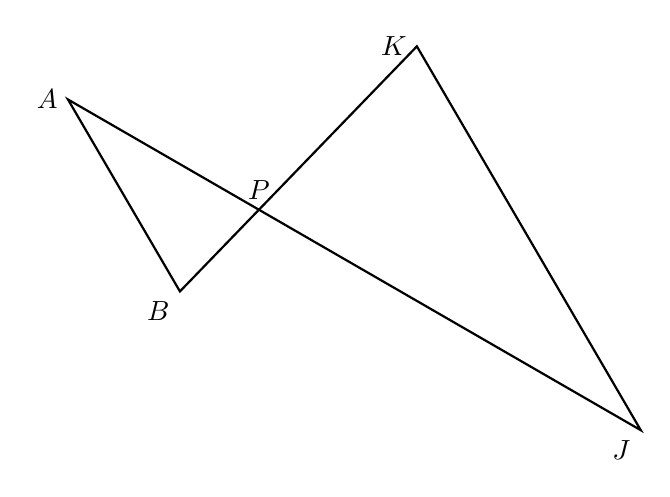
\begin{tikzpicture}[rotate=-30, scale=1.4]
        \draw [thick]
          (-0.25,-1)node[below left]{$B$}--
          (0.5,2)node[left]{$K$}--
          (4,0)node[below left]{$J$}--
          (0,0)node[above]{$P$}--
          (-2,0)node[left]{$A$}--cycle;
      \end{tikzpicture}
    \end{multicols}
      \vspace{1cm}

  \item Given $\triangle PQR \sim \triangle STU$, $m\angle P=37^\circ$, and $m\angle T=46^\circ$. Find $m\angle Q$. \vspace{3cm}

  \begin{multicols}{2}[\item The diagram below shows $\triangle ABC$, with $\overline{AEB}$ and $\overline{ADC}$.]
    \begin{enumerate}
      \item Justify $\angle BAC \cong \angle DAE$.
      \item What angle must be congruent to $\angle AED$ to prove $\triangle ABC \sim \triangle ADE$ by \emph{angle-angle similarity}? \vspace{3cm}
    \end{enumerate}
      \begin{tikzpicture}[scale=1.3]
        \draw [thick]
        (0,0) node[above right] {$A$}--
        (230:6) node[below left] {$B$}--
        (260:4.75) node[below right] {$C$}--cycle;
        \draw [thick]
        (230:2.375) node[above left] {$E$}--
        (260:3) node[right] {$D$}--cycle;
      \end{tikzpicture}
    \end{multicols}

\newpage
  \item In $\triangle ABC$ shown below, $\angle ACB$ is a right angle, $E$ is a point on $\overline{AC}$, and $\overline{ED}$ is drawn perpendicular to hypontenuse $\overline{AB}$.
    \begin{center}
      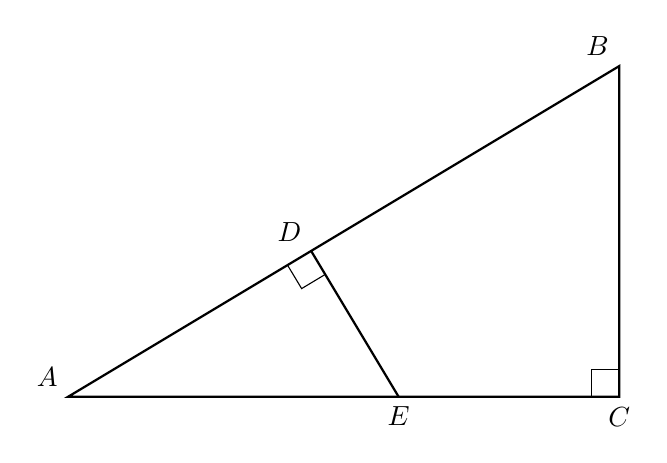
\begin{tikzpicture}[scale=0.7]
        \draw [-, thick] (0,0) node[above left]{$A$}--
        (10,0) node[below]{$C$}--
        (10,6) node[above left]{$B$}--cycle;
        \draw [thick] (6,0)--(4.41,2.65);
        \node at (6,0) [below]{$E$};
        \node at (4.41,2.65) [above left]{$D$};
        \draw (10,0) ++(-0.5,0)--++(0,0.5)--++(0.5,0);
        \draw (4.41,2.65) ++(-59:0.5)--++(-149:0.5)--++(121:0.5);
        %\node at (4, 0) [below]{$12$};
        %\node at (3,2) [above]{$9$};
        %\node at (9, 3) [right]{$10$};
        %\node at (5.5, 1.6) [right]{$6$}; \vspace{1cm}
      \end{tikzpicture}
    \end{center} 
    If $AB = 9$, $BC = 6$, and $DE = 4$, what is the length of $\overline{AE}$? \vspace{3cm}

  \item In the diagram below, the chords $\overline{AE}$ and $\overline{BD}$ intersect at $C$. Given  $AC=6$, $BC=4$, and $EC=7$.
  \begin{multicols}{2}
    \begin{enumerate}[itemsep=1cm]
      \item What angle corresponds with $\angle D$?
      \item Complete the similarity statement: $\triangle ABC \sim$
      \item Determine the length of $\overline{CD}$. \vspace{3cm}
    \end{enumerate}
      \begin{flushright}
      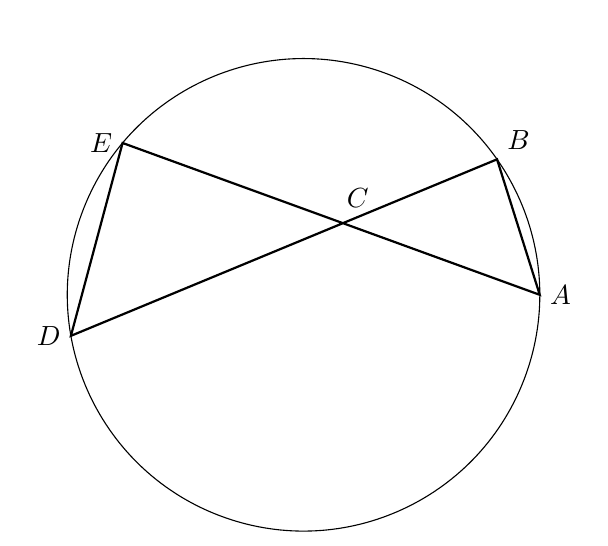
\begin{tikzpicture}[rotate=-20, scale=.6]
        \draw (0,0) circle[radius=5];
        \draw [thick]
        (20:5) node[right] {$A$}--
        (160:5) node[left] {$E$}--
        (210:5) node[left] {$D$}--
        (55:5) node[above right] {$B$}--cycle;
        \draw (75:2) node[above] {$C$};
      \end{tikzpicture}
    \end{flushright}
  \end{multicols}

\end{enumerate}
\end{document}